\documentclass[10pt,a4paper]{article}
\usepackage[UTF8,fontset = windows]{ctex}
\setCJKmainfont[BoldFont=黑体,ItalicFont=楷体]{华文中宋}
\usepackage{amssymb,amsmath,amsfonts,amsthm,mathrsfs,dsfont,graphicx}
\usepackage{ifthen,indentfirst,enumerate,color,titletoc}
\usepackage{tikz}
\usetikzlibrary{arrows,calc,intersections}
\usepackage[bf,small,indentafter,pagestyles]{titlesec}
\usepackage[top=1in, bottom=1in,left=0.8in,right=0.8in]{geometry}
\renewcommand{\baselinestretch}{1.65}
\newtheorem{defi}{定义~}
\newtheorem{eg}{例~}
\newtheorem{ex}{~}
\newtheorem{rem}{注~}
\newtheorem{thm}{定理~}
\newtheorem{coro}{推论~}
\newtheorem{axiom}{公理~}
\newtheorem{prop}{性质~}

\newcommand{\blank}[1]{\underline{\hbox to #1pt{}}}
\newcommand{\bracket}[1]{(\hbox to #1pt{})}

\newcommand{\onech}[4]{\par\begin{tabular}{p{.9\textwidth}}
A.~#1\\
B.~#2\\
C.~#3\\
D.~#4
\end{tabular}}

\newcommand{\twoch}[4]{\par\begin{tabular}{p{.46\textwidth}p{.46\textwidth}}
A.~#1& B.~#2\\
C.~#3& D.~#4
\end{tabular}}

\newcommand{\vartwoch}[4]{\par\begin{tabular}{p{.46\textwidth}p{.46\textwidth}}
(1)~#1& (2)~#2\\
(3)~#3& (4)~#4
\end{tabular}}


\newcommand{\fourch}[4]{\par\begin{tabular}{p{.23\textwidth}p{.23\textwidth}p{.23\textwidth}p{.23\textwidth}}
A.~#1 &B.~#2& C.~#3& D.~#4
\end{tabular}}

\newcommand{\varfourch}[4]{\par\begin{tabular}{p{.23\textwidth}p{.23\textwidth}p{.23\textwidth}p{.23\textwidth}}
(1)~#1 &(2)~#2& (3)~#3& (4)~#4
\end{tabular}}
    

\begin{document}
2022届高三冲刺题

\begin{enumerate}[1.]
\item 已知函数$f(x)=\log_a x+x-b$($a>0$且$a\ne 1$). 当$2<a<3<b<4$时, 函数$f(x)$的零点$x_0\in (n,n+1), \ n\in \mathbf{N}^*$, 则$n=$\blank{50}.
\item 设实数$a,b,c$满足: $ac\ne 0$且$a\ne c$, 集合$A=\{y|y=ax^2+bx+c, \ x\in \mathbf{R}\}$, $B=\{y|y=cx^2+bx+a\}$, 以下结论一定正确的是\bracket{20}.
\fourch{$A\subseteq B$}{$B\subseteq A$}{$A\cup B=\mathbf{R}$}{$A\cap B\ne\varnothing$}
\item 对于无穷数列$\{a_n\}$, 定义数列$b_n=|a_{n+1}-a_n|$, 记$\{b_n\}$的前$n$项和为$S_n$, 若$\displaystyle\lim_{n\to \infty} S_n$存在, 则称数列$\{a_n\}$为``好数列''.\\
(1) 若$a_n=\dfrac{1}{n}$, 判断数列$\{a_n\}$是否为``好数列''? 并说明理由;\\
(2) 若数列$\{a_n\}$满足$a_1=1$, $a_{n+1}=qa_n \ (q\ne 0)$, 且$\{a_n\}$是``好数列'', 求$q$的取值范围;\\
(3) 若递增数列$\{a_n\}$的前$n$项和为$\{T_n\}$, 则``$\{a_n\}$为`好数列'''是``$\{T_n\}$为`好数列'''的什么条件? 判断并说明理由.
\item 函数$f(x)=\sin x$, 对于$x_1<x_2<x_3<\cdots<x_n$且$x_1,x_2,\cdots,x_n\in [0,8\pi] \ (n\ge 10, \ n\in \mathbf{N})$, 记$M=|f(x_1)-f(x_2) |+|f(x_2)-f(x_3)|+|f(x_3)-f(x_4)|+\cdots+| f(x_{n-1})-f(x_n)|$, 则$M$的最大值等于\blank{50}. 
\item 设$\alpha_1,\alpha_2\in \mathbf{R}$, 且$\dfrac1{2+\sin\alpha_1}+\dfrac1{2+\sin(2\alpha_2)}=2$, 则$|10 \pi-\alpha_1-\alpha_2|$的最小值等于\blank{50}.
\item 正四棱锥$V-ABCD$的表面积为$12$, $AB=2$, $N$为棱$CD$的中点, 直线$AB$在平面$\alpha$内. 将该正四棱锥绕直线$AB$任意旋转, 旋转过程中, 设$V$在$\alpha$内的射影为$O$, 则线段$ON$长的最大值为\blank{50}.
\begin{center}
    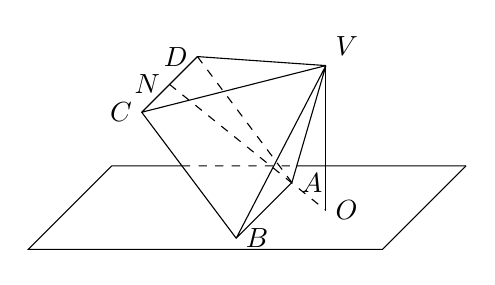
\begin{tikzpicture}
        \coordinate (V) at ({4*sqrt(3)/5},{3*sqrt(3)/5});
        \coordinate (A) at ({3/5+sqrt(2)/4},{-4/5+sqrt(2)/4});
        \coordinate (B) at ({3/5-sqrt(2)/4},{-4/5-sqrt(2)/4});
        \coordinate (C) at ({-3/5-sqrt(2)/4},{4/5-sqrt(2)/4});
        \coordinate (D) at ({-3/5+sqrt(2)/4},{4/5+sqrt(2)/4});
        \draw (V) node [above right] {$V$} -- (A) node [right] {$A$} -- (B) node [right] {$B$} -- (C) node [left] {$C$} -- (D) node [left] {$D$}  (V) -- (B) (V) -- (C) (V) -- (D);
        \draw [dashed] (D) -- (A); 
        \draw (V) -- ({4*sqrt(3)/5},{-4/5}) coordinate (O) node [right] {$O$};
        \draw (B) ++ (225:0.2) ++ (-2.5,0) coordinate (P);
        \draw (P) ++ (4.5,0) coordinate (Q);
        \draw (Q) ++ (45:1.5) coordinate (T) ++ (-4.5,0) coordinate (S);
        \draw (S) -- (P) -- (Q) -- (T);
        \draw ($(C)!0.5!(D)$) node [left] {$N$} coordinate (N);
        \path [name path=A--V] (A) -- (V);
        \path [name path=S--T] (S) -- (T);
        \path [name path=B--C] (B) -- (C);
        \path [name intersections={of = A--V and S--T,by=F}];
        \path [name intersections={of = B--C and S--T,by=E}];
        \draw (S) -- (E) (F) -- (T);
        \draw [dashed] (E) -- (F);
        \draw [dashed] (N) -- (O);
    \end{tikzpicture}
\end{center}
\item 已知$a,b$为空间两条互相垂直的直线, 等腰$\mathrm{Rt}\triangle ABC$的直角边$AC$所在直线与$a,b$都垂直, 斜边$AB$以直线$AC$为旋转轴旋转. 有下列结论: \textcircled{1} 当直线$AB$与$a$所成的角为$60^\circ$时, $AB$与$b$所成的角为$30^\circ$; \textcircled{2} 直线$AB$与$a$所成角的最小值为$45^\circ$; \textcircled{3} 直线$AB$与$a$所成角的最大值为$60^\circ$. 其中所有真命题的序号为\blank{50}.
\item 已知数列$\{a_n\}$满足: \textcircled{1} $a_1=0$; \textcircled{2} 对任意的$n\in \mathbf{N}^*$, 都有$a_{n+1}>a_n$成立. 
函数$f_n(x)=|\sin \dfrac{1}{n}(x-a_n)|, \ x\in [a_n,a_{n+1}]$满足: 对于任意的实数$m\in [0,1)$, $f_n(x)=m$总是有且仅有两个不同的根, 求$\{a_n\}$的通项公式.
\item 设$\overrightarrow a,\overrightarrow b,\overrightarrow c$是平面上的向量,$|\overrightarrow a| =1,|\overrightarrow b| =3,|\overrightarrow c|=4$, 且$\overrightarrow b\cdot \overrightarrow c=0$, 实数$\lambda$满足$0 \le \lambda \le 1$. 若$\overrightarrow a,\overrightarrow b,\overrightarrow c$及$\lambda$, 使得$s=|\overrightarrow a-\lambda \overrightarrow b-(1-\lambda)\overrightarrow c|$是正整数, 则$s$的值的集合是\blank{50}.
\item 如图, 在平面内, $l_1,l_2$是两条平行直线, 它们之间的距离为$2$, 点$P$位于$l_1,l_2$的下方, 它到$l_1$的距离为$1$, 动点$N,M$分别在$l_1,l_2$上, 满足$|\overrightarrow{PM}+\overrightarrow{PN}|=6$, 则$\overrightarrow{PM}\cdot \overrightarrow{PN}$的最大值为\bracket{20}.
\fourch{$6$}{$8$}{$12$}{$15$}
\begin{center}
    \begin{tikzpicture}[>=latex]
        \draw (0,0) -- (5,0) node [right] {$l_1$} (0,2) -- (5,2) node [right] {$l_2$};
        \draw [->] (4.5,-1) node [below right] {$P$} -- (2,0) node [below] {$N$};
        \draw [->] (4.5,-1) -- (2.5,2) node [below] {$M$};
    \end{tikzpicture}
\end{center}
\item 已知过原点$O$的直线与椭圆$C:\dfrac{x^2}4+{y^2}=1$交于$A,B$两点, 点$A$到$y$的距离$d$满足$d\in [1,2)$, 点$D$在椭圆$C$上, 且$AD\perp AB$, 直线$BD$与$x$轴、$y$轴分别交于$M,N$两点.\\
(1) 设直线$BD,AM$的斜率分别为$k_1,k_2$, 求$k_1\cdot k_2$的取值范围;  
(2) 求$\triangle OMN$面积的最大值.
\item 已知点$A(0,\dfrac2n)$, $B(0,-\dfrac2n)$, $C(4+\dfrac2n,0)$, 其中$n$为正整数, 设$S_n$表示$\triangle ABC$外接圆的面积, 则$\displaystyle\lim_{n\to\infty}{S_n}=$\blank{50}.
\item 如图所示: 矩形$A_nB_nP_nQ_n$的一边$A_nB_n$在$x$轴上, 另两个顶点$P_n,Q_n$在函数$f(x)=\dfrac{2x}{1+x^2}$的图像上(其中点$B_n$的坐标为$(n,0) \ (n\ge 2,\ n\in \mathbf{N}^*)$), 矩形$A_nB_nP_nQ_n$的面积记为$S_n$, 则$\displaystyle\lim_{n\to\infty}{S_n}=$\blank{50}.
\begin{center}
    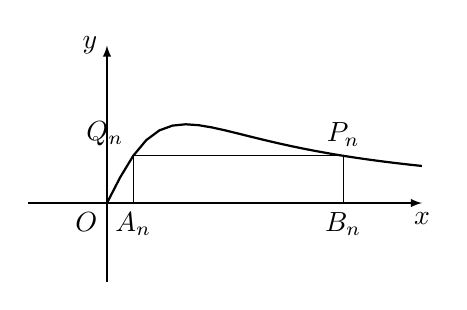
\begin{tikzpicture}[>=latex]
        \draw [->] (-1,0) -- (4,0) node [below] {$x$};
        \draw [->] (0,-1) -- (0,2) node [left] {$y$};
        \draw (0,0) node [below left] {$O$};
        \draw [thick, domain = 0:4] plot (\x,{2*\x/(1+\x*\x)});
        \draw ({1/3},0) node [below] {$A_n$} -- ({1/3},{3/5}) node [above left] {$Q_n$} -- (3,{3/5}) node [above] {$P_n$} -- (3,0) node [below] {$B_n$};
    \end{tikzpicture}
\end{center}
\end{enumerate}
\end{document}